


\tikzset{every picture/.style={line width=0.75pt}} %set default line width to 0.75pt        

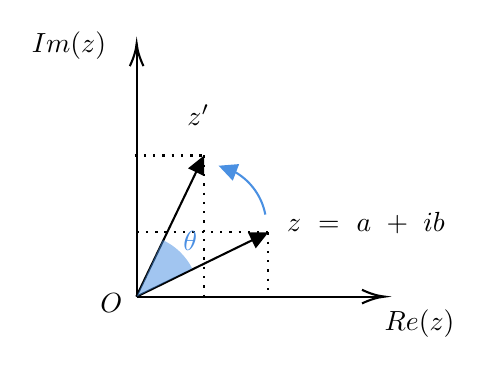
\begin{tikzpicture}[x=0.75pt,y=0.75pt,yscale=-1,xscale=1]
%uncomment if require: \path (0,15225); %set diagram left start at 0, and has height of 15225

%Straight Lines [id:da5015611160293443] 
\draw    (526,6086) -- (643.5,6086) ;
\draw [shift={(645.5,6086)}, rotate = 180] [color={rgb, 255:red, 0; green, 0; blue, 0 }  ][line width=0.75]    (10.93,-3.29) .. controls (6.95,-1.4) and (3.31,-0.3) .. (0,0) .. controls (3.31,0.3) and (6.95,1.4) .. (10.93,3.29)   ;
%Straight Lines [id:da7739785169188371] 
\draw    (526,6086) -- (526,5966) ;
\draw [shift={(526,5964)}, rotate = 90] [color={rgb, 255:red, 0; green, 0; blue, 0 }  ][line width=0.75]    (10.93,-3.29) .. controls (6.95,-1.4) and (3.31,-0.3) .. (0,0) .. controls (3.31,0.3) and (6.95,1.4) .. (10.93,3.29)   ;
%Straight Lines [id:da6097015977657645] 
\draw  [dash pattern={on 0.84pt off 2.51pt}]  (526,6055) -- (589.5,6055) ;
%Straight Lines [id:da06830863122513897] 
\draw  [dash pattern={on 0.84pt off 2.51pt}]  (589.5,6055) -- (589.5,6086) ;
%Straight Lines [id:da1339436079722769] 
\draw    (526,6086) -- (586.8,6056.32) ;
\draw [shift={(589.5,6055)}, rotate = 153.98] [fill={rgb, 255:red, 0; green, 0; blue, 0 }  ][line width=0.08]  [draw opacity=0] (8.93,-4.29) -- (0,0) -- (8.93,4.29) -- cycle    ;
%Straight Lines [id:da12876867450395124] 
\draw    (525.83,6086) -- (557.2,6020.7) ;
\draw [shift={(558.5,6018)}, rotate = 115.66] [fill={rgb, 255:red, 0; green, 0; blue, 0 }  ][line width=0.08]  [draw opacity=0] (8.93,-4.29) -- (0,0) -- (8.93,4.29) -- cycle    ;
%Straight Lines [id:da6964942743081263] 
\draw  [dash pattern={on 0.84pt off 2.51pt}]  (525,6018) -- (558.5,6018) ;
%Straight Lines [id:da21207065554446136] 
\draw  [dash pattern={on 0.84pt off 2.51pt}]  (558.5,6018) -- (558.5,6086) ;
%Straight Lines [id:da7448312272789616] 
\draw [color={rgb, 255:red, 74; green, 144; blue, 226 }  ,draw opacity=1 ]   (573.49,6026.01) -- (568.31,6024.02) ;
\draw [shift={(565.51,6022.94)}, rotate = 21.06] [fill={rgb, 255:red, 74; green, 144; blue, 226 }  ,fill opacity=1 ][line width=0.08]  [draw opacity=0] (8.93,-4.29) -- (0,0) -- (8.93,4.29) -- cycle    ;
%Shape: Arc [id:dp7227532122430883] 
\draw  [draw opacity=0] (573.49,6026.01) .. controls (580.94,6030.31) and (586.36,6037.72) .. (587.99,6046.47) -- (558.5,6052) -- cycle ; \draw  [color={rgb, 255:red, 74; green, 144; blue, 226 }  ,draw opacity=1 ] (573.49,6026.01) .. controls (580.94,6030.31) and (586.36,6037.72) .. (587.99,6046.47) ;  
%Shape: Arc [id:dp5675882433264926] 
\draw  [draw opacity=0][fill={rgb, 255:red, 74; green, 144; blue, 226 }  ,fill opacity=0.52 ] (538.61,6058.77) .. controls (544.71,6061.6) and (549.7,6066.42) .. (552.75,6072.4) -- (526,6086) -- cycle ; \draw  [draw opacity=0] (538.61,6058.77) .. controls (544.71,6061.6) and (549.7,6066.42) .. (552.75,6072.4) ;  

% Text Node
\draw (474,5957) node [anchor=north west][inner sep=0.75pt]    {$Im( z)$};
% Text Node
\draw (597,6044) node [anchor=north west][inner sep=0.75pt]    {$z\ =\ a\ +\ ib$};
% Text Node
\draw (644,6091) node [anchor=north west][inner sep=0.75pt]    {$Re( z)$};
% Text Node
\draw (507,6083) node [anchor=north west][inner sep=0.75pt]    {$O$};
% Text Node
\draw (549,5992) node [anchor=north west][inner sep=0.75pt]    {$z'$};
% Text Node
\draw (547,6053) node [anchor=north west][inner sep=0.75pt]    {$\textcolor[rgb]{0.29,0.56,0.89}{\theta }$};


\end{tikzpicture}